
\documentclass{beamer}

\usetheme{default}
\usepackage{tikz}
\usetikzlibrary{arrows,shapes.arrows,positioning,shapes}
\usepackage{graphicx}
\usepackage{hyperref}
\newcommand\red[1]{{\color{red}#1}}
\newcommand\bred[1]{{\color{red}\textbf{#1}}}
\newcommand\blue[1]{{\color{blue}#1}}
\newcommand\bblue[1]{{\color{blue}\textbf{#1}}}
\newcommand\green[1]{{\color{olive}#1}}
\newcommand\bgreen[1]{{\color{olive}\textbf{#1}}}
\newcommand\black[1]{{\color{black}#1}}
\newcommand\white[1]{{\color{white}#1}}
\newcommand\E{\text{E}}
\newcommand\V{\text{V}}
\renewcommand\P{\text{P}}
\def\checkmark{\tikz\fill[olive, scale=0.6](-.125,.375) -- (.25,0) -- (1.125,.875) -- (1, 1) -- (.25,.25) -- (0,.5) -- cycle;} 
\def\circlecheckmark{

\begin{tikzpicture}[scale = .6]
\fill[olive](-.125,.375) -- (.25,0) -- (1.125,.875) -- (1, 1) -- (.25,.25) -- (0,.5) -- cycle;
\draw[olive, line width = .1cm] (0.5,0.5) ellipse (0.9 and 0.9);
\end{tikzpicture}
} 
\def\bigx{
\begin{tikzpicture}[x=.4cm,y=.4cm]
\draw[thick, line width = .1cm, red] (0,0) -- (1,1); 
\draw[thick, line width = .1cm, red] (0,1) -- (1,0);
\end{tikzpicture}} 
\usepackage{array}
\usepackage{soul}
\newcolumntype{V}{>{\centering\arraybackslash} m{.12\linewidth}}
\newcolumntype{B}[1]{>{\centering\arraybackslash}b{#1}}

\newcommand{\indep}{{\bot\negthickspace\negthickspace\bot}}

\title{Privacy, ethics, and data access:\\ \normalsize A case study of the Fragile Families Challenge \vspace{-.2in}}

\author{\small Ian Lundberg, Arvind Narayanan, Karen Levy, and Matthew J. Salganik \vspace{-.05in}}

\institute[]
{
  Department of Sociology, Office of Population Research, \& \\Center for Research on Child Wellbeing, Princeton University}

\date{Aug. 12, 2018\\Annual Meeting of the American Sociological Association\\
\begin{flushleft}{\scriptsize
This research is supported by the Russell Sage Foundation.  We are grateful to the members of the Board of Advisors of the Fragile Families Challenge: Jeanne Brooks-Gunn, Kathryn J. Edin, Barbara E. Engelhardt, Irwin Garfinkel, Moritz Hardt, Dean Knox, Nicholas Lemann, Karen Levy, Sara McLanahan, Arvind Narayanan, Timothy J. Nelson, Matthew Salganik, \& Duncan Watts.  Source for these slides: \textcolor{blue}{\textcolor{blue}{\href{http://github.com/fragilefamilieschallenge}{www.github.com/fragilefamilieschallenge}}}. \includegraphics[width=0.05\textwidth]{figures/cc.png}}
\end{flushleft}
}

%\pgfdeclareimage[height=1cm]{university-logo}{ff_logo.jpg}
%\logo{\pgfuseimage{university-logo}}

%%%%%%%%%%%%%%%%%%%%%%%%%%%%%%
\begin{document}

%\begin{frame}
%  \titlepage
%\end{frame}

\begin{frame}
\centering
\begin{tikzpicture}[x = .5\textwidth, y = .5\textwidth]
\node at (-1,-1) {};
\node at (1,1) {};
\node[font = \Huge, blue] at (-.35, .8) {Privacy, ethics};
\node[font = \Huge, blue] at (-.35, .65) {and data access};
\node[font = \huge, olive, align = center] at (-.35, .3) {A case study of the\\Fragile Families Challenge};
\node[align = center] at (-.45, -.15) {Ian Lundberg\\Arvind Narayanan\\Karen Levy\\Matthew J. Salganik};
\node[align=center,font = \footnotesize, darkgray] (sociology) at (-.9, -.15) {Sociology\\Princeton};
\draw[->, thick, darkgray] (sociology) to[bend left] (-.68, 0);
\draw[->, thick, darkgray] (sociology) to[bend right] (-.8, -.28);
\node[align=center,font = \footnotesize, darkgray] (cs) at (.2, -.05) {Computer Science\\Princeton};
\draw[->, thick, darkgray] (cs) -- (-.17, -.1);
\node[align=center,font = \footnotesize, darkgray] (is) at (.2, -.25) {Information Science\\Cornell};
\draw[->, thick, darkgray] (is) -- (-.22, -.2);
\node[align = center] at (-.45, -.45) {13 August 2018};
\node[align = center] at (-.45, -.6) {Annual Meeting of the\\American Sociological Association};
\node[align = center, anchor = north east, font = \scriptsize] at (1.05, 1) {\begin{minipage}{.3\textwidth}\begin{flushright}This research is supported by the Russell Sage Foundation.  We are grateful to the members of the Board of Advisors of the Fragile Families Challenge%: Jeanne Brooks-Gunn, Kathryn J. Edin, Barbara E. Engelhardt, Irwin Garfinkel, Moritz Hardt, Dean Knox, Nicholas Lemann, Karen Levy, Sara McLanahan, Arvind Narayanan, Timothy J. Nelson, Matthew Salganik, \& Duncan Watts
.  Source for these slides: \textcolor{blue}{\textcolor{blue}{\href{http://github.com/fragilefamilieschallenge}{www.github.com/\\fragilefamilieschallenge}}}.\\\includegraphics[width=0.4\textwidth]{figures/cc.png}\end{flushright}\end{minipage}};
\end{tikzpicture}
\end{frame}

\begin{frame}
\begin{figure}
\centering
\includegraphics[width=.8\textwidth]{figures/tensionFig}
\end{figure}
\end{frame}

\begin{frame}
\begin{figure}
\centering
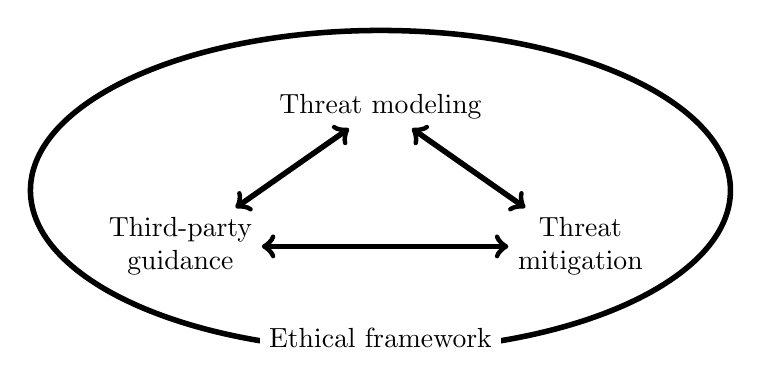
\begin{tikzpicture}[x = 1in, y = .7in]
\node (threatModeling) at (0,1) {Threat modeling};
\node[align=center] (threatMitigation) at (1,0) {Threat\\mitigation};
\node[align=center] (third) at (-1,0) {Third-party\\guidance};
% Triangle edges
\draw[<->,line width = 2pt] (threatModeling) -- (threatMitigation);
\draw[<->,line width = 2pt] (third) -- (threatMitigation);
\draw[<->,line width = 2pt] (third) -- (threatModeling);
\draw[line width = 2pt] (0,.4) ellipse (1.75in and .8in);
\node[fill=white] at (0, -.65) {Ethical framework};
\end{tikzpicture}
\label{fig:process}
\end{figure}
\end{frame}

\begin{frame}
\begin{tikzpicture}[x = .5\textwidth, y = .5\textwidth]
\node[anchor = north] at (0,1) {\includegraphics[width=\textwidth]{figures/ff_logo}};
\onslide<1-1>{
\node[anchor = north west] at (-.8,.4) {\vbox{\begin{itemize}
\item Birth cohort panel study
\item $\approx$ 5,000 children born in 20 U.S. cities
\item Followed from birth through age 15
\end{itemize}}};
}
\onslide<2->{
\node[anchor = north west] at (-.9,.4) {Features relevant to privacy:};
\node[anchor = north west] at (-.8,.3) {\vbox{\begin{enumerate}
\item Informed consent
\onslide<3->{\item Already available to researchers}
\onslide<4->{\item Already used in scientific and policy debates}
\onslide<5->{\item Contain information from many respondents}
\end{enumerate}}};
}
\end{tikzpicture}
\end{frame}
%%%%%%%%%%%%%%%%%%%%%%%%%
\begin{frame}

\begin{center}
%\includegraphics[height=0.8\textheight]<1>{figures/ff_design_public_b9}
\includegraphics[height=0.8\textheight]{figures/ff_design_public_b9_15}
\end{center}

\end{frame}
%%%%%%%%%%%%%%%%%%%%%%%%%
\begin{frame}

\begin{center}
%\includegraphics[width=\textwidth]{figures/ff_design_matrix_ml}
\includegraphics[width=\textwidth]{figures/ffc_design_matrix_ml}
\end{center}

\end{frame}
%%%%%%%%%%%%%%%%%%%%%%%%%

\begin{frame}
\centering
{\Large The Princeton IRB approved the project. \pause \vskip .2cm The data met standards for de-identification. \pause \vskip .5cm}
{\huge \bblue{Why worry?}}
\end{frame}

\begin{frame}
\centering
\includegraphics[width = .4\textwidth]{figures/LexLuthor}\\Art by David Finch\\Source: Wikipedia
\end{frame}

\begin{frame}
\centering
A. Sweeney (1997) re-identified Massachusetts medical records \vskip .4cm
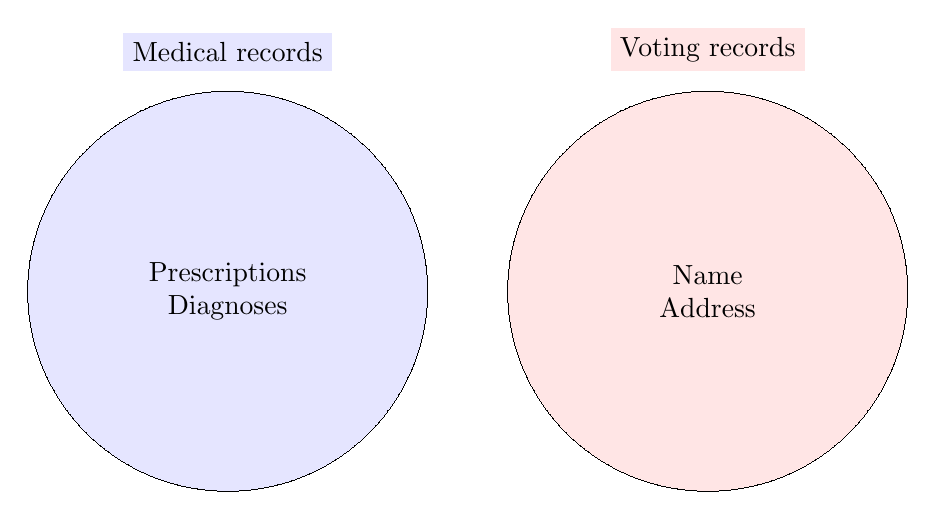
\begin{tikzpicture}[x = 1in, y = 1in]
\draw[blue, fill=blue, draw = black, fill opacity = .1, line width = 0pt] (-.2,0) ellipse (1in and 1in);
\draw[red, fill=red, draw = black, fill opacity = .1, line width = 0pt] (2.2,0) ellipse (1in and 1in);
\node[align=center] at (-.2,0) {Prescriptions\\Diagnoses};
\node[align=center] at (2.2,0) {Name\\Address};
\node[align=center,fill = blue, fill opacity = .1, text opacity = 1, anchor=south] at (-0.2,1.1) {Medical records};
\node[align=center,fill = red, fill opacity = .1, text opacity = 1, anchor=south] at (2.2,1.1) {Voting records};
\end{tikzpicture}
\end{frame}

\begin{frame}
\centering
A. Sweeney (1997) re-identified Massachusetts medical records \vskip .4cm
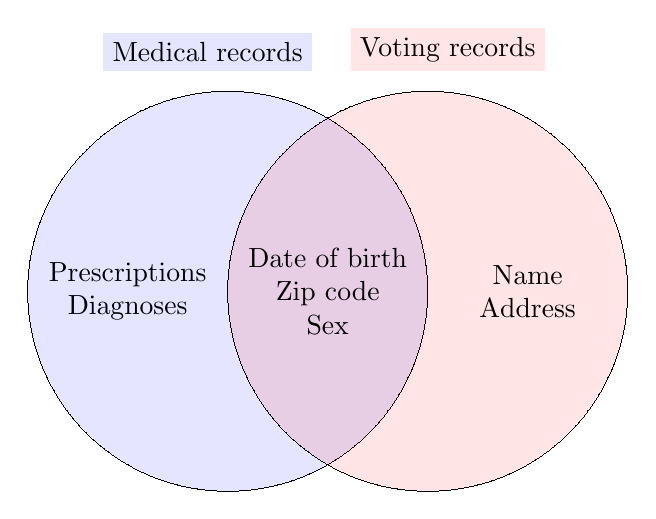
\begin{tikzpicture}[x = 1in, y = 1in]
\draw[blue, fill=blue, draw = black, fill opacity = .1, line width = 0pt] (0.5,0) ellipse (1in and 1in);
\draw[red, fill=red, draw = black, fill opacity = .1, line width = 0pt] (1.5,0) ellipse (1in and 1in);
\node[align=center] at (0,0) {Prescriptions\\Diagnoses};
\node[align=center] at (2,0) {Name\\Address};
\node[align=center] at (1,0) {Date of birth\\Zip code\\Sex};
\node[align=center,fill = blue, fill opacity = .1, text opacity = 1, anchor=south] at (0.4,1.1) {Medical records};
\node[align=center,fill = red, fill opacity = .1, text opacity = 1, anchor=south] at (1.6,1.1) {Voting records};
\end{tikzpicture}
\end{frame}

\begin{frame}
B. Malin and Sweeney (2004) re-identified genomics data
\begin{center}
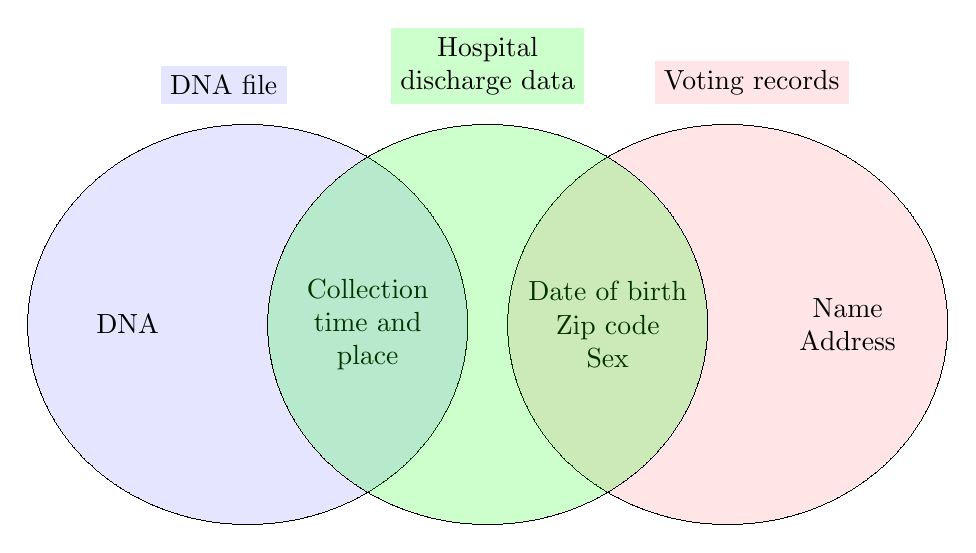
\begin{tikzpicture}[x = 1.2in, y = 1in]
\draw[blue, fill=blue, draw = black, fill opacity = .1, line width = 0pt] (0.5,0) ellipse (1.1in and 1in);
\draw[red, fill=red, draw = black, fill opacity = .1, line width = 0pt] (2.5,0) ellipse (1.1in and 1in);
\node[align=center] at (0,0) {DNA};
\node[align=center] at (1,0) {Collection\\time and\\place};
\node[align=center] at (2,0) {Date of birth\\Zip code\\Sex};
\only<2-2>{
\node[align=center,fill=green, fill opacity = .2, text opacity = 1, anchor=south] at (1.5,1.1) {Hospital\\discharge data};
\draw[yellow, fill=green, draw = black, fill opacity = .2, line width = 0pt] (1.5,0) ellipse (1.1in and 1in);
}
\node[align=center] at (3,0) {Name\\Address};
\node[align=center,black,fill=blue,fill opacity = .1, text opacity = 1, anchor=south] at (0.4,1.1) {DNA file};
\node[align=center,fill = red, fill opacity = .1, text opacity = 1, anchor=south] at (2.6,1.1) {Voting records};
\end{tikzpicture}
\end{center}
\end{frame}

\begin{frame}
{\large C. We don't know the auxiliary data that may exist.}
\begin{figure}
\centering
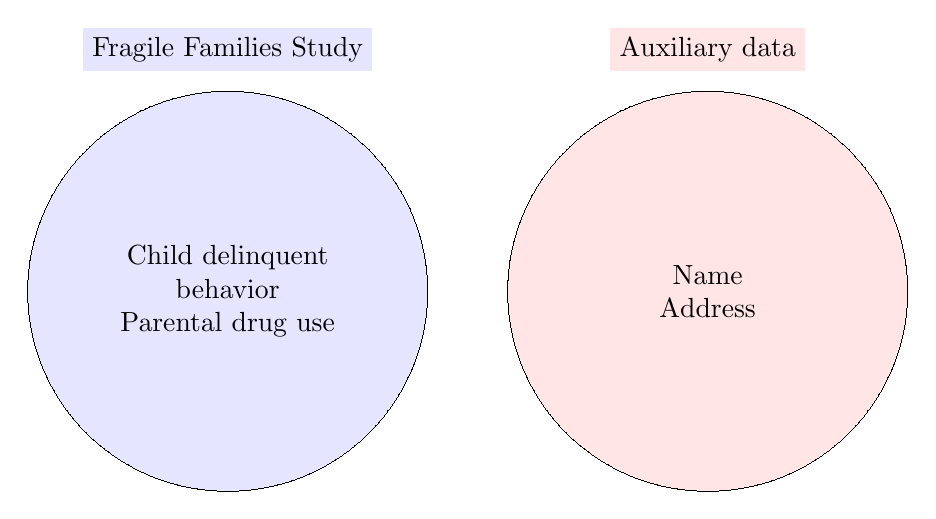
\begin{tikzpicture}[x = 1.5in, y = 1in]
\draw[blue, fill=blue, draw = black, fill opacity = .1, line width = 0pt] (0.2,0) ellipse (1in and 1in);
\draw[red, fill=red, draw = black, fill opacity = .1, line width = 0pt] (1.8,0) ellipse (1in and 1in);
\node[align=center] at (.2,0) {Child delinquent\\behavior\\ Parental drug use};
\node[align=center] at (1.8,0) {Name\\Address};
\node[align=center,fill = blue, fill opacity = .1, text opacity = 1, anchor=south] at (0.2,1.1) {Fragile Families Study};
\node[align=center,fill = red, fill opacity = .1, text opacity = 1, anchor=south] at (1.8,1.1) {Auxiliary data};
\end{tikzpicture}
\end{figure}
\end{frame}

\begin{frame}
{\large C. We don't know the auxiliary data that may exist.}
\begin{figure}
\centering
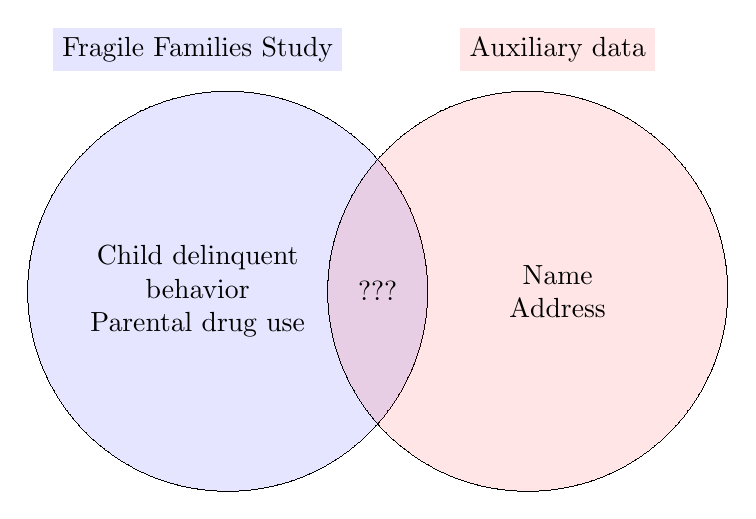
\begin{tikzpicture}[x = 1.5in, y = 1in]
\draw[blue, fill=blue, draw = black, fill opacity = .1, line width = 0pt] (0.5,0) ellipse (1in and 1in);
\draw[red, fill=red, draw = black, fill opacity = .1, line width = 0pt] (1.5,0) ellipse (1in and 1in);
\node[align=center] at (.4,0) {Child delinquent\\behavior\\ Parental drug use};
\node[align=center] at (1.6,0) {Name\\Address};
\node[align=center] at (1,0) {???};
\node[align=center,fill = blue, fill opacity = .1, text opacity = 1, anchor=south] at (0.4,1.1) {Fragile Families Study};
\node[align=center,fill = red, fill opacity = .1, text opacity = 1, anchor=south] at (1.6,1.1) {Auxiliary data};
\end{tikzpicture}
\end{figure}
\end{frame}

\begin{frame}{Provable privacy protections}

Promising areas of active research:
\begin{itemize}
\item Differential privacy
\item Cryptography
\end{itemize}
\begin{center}
\pause

\begin{tikzpicture}
\node[align = center] at (-3.3, 0) {At their present development,\\neither applied in our setting.}; \pause
\draw[->, line width = 2pt, blue] (-.5,0) -- (1,0);
\node[align = center] at (3.3, 0) {Turned to approaches\\without\\provable guarantees.};
\end{tikzpicture}

\end{center}

\end{frame}

\begin{frame}{Threat modeling}
\bblue{Criteria} that represent a threat of a re-identification attack:
\begin{itemize}
\item skills
\item auxiliary data
\item incentives
\end{itemize} \vskip .2cm \pause
\bblue{Concrete experience:} We attacked our own data for 1.5 months. \vskip .2cm \pause
\bblue{Main threats:}
\begin{enumerate}
\item Privacy researcher* \pause
\item Nosy neighbor \pause
\item Troll \pause
\item Journalist \pause 
\item Cheater
\end{enumerate}
\end{frame}

\newcommand{\mitigations}{\begin{frame}
\begin{tikzpicture}
\node[rotate = 90, blue, font= \bf] at (-5.5, 0) {$\leftarrow$ Threats $\rightarrow$};
\node[blue, font= \bf] at (1,3.8) {$\leftarrow$ Mitigations $\rightarrow$};
\node at (0,0) {\vbox{
\begin{table}
\resizebox{\textwidth}{!}{
\begin{tabular}{m{.65in}VVVVVV}
& Low & Careful & Challenge & Application  & Ethical & Modifications\\
& profile & language & structure & process & appeal & to data \\
\hline
Privacy researcher & \checkmark & \circlecheckmark & \checkmark & \checkmark & \checkmark & \checkmark \\
Nosy neighbor & \circlecheckmark & & & \checkmark & & \\
Troll & \circlecheckmark &  & \checkmark & \checkmark &  & \checkmark \\
Journalist & \checkmark & \checkmark & \checkmark & \circlecheckmark & \checkmark & \checkmark \\
Cheater &  & \checkmark & \circlecheckmark &  & \checkmark & \checkmark
\end{tabular}
}
\end{table}
}};
\end{tikzpicture}
\end{frame}
}

\mitigations

\begin{frame}{Response plan}
We mitigated but did not eliminate risks. \vskip .5cm
We needed a team ready to respond in a crisis
\begin{itemize}
\item Computer scientist who had re-identified datasets previously
\item Lawyer and sociologist who studies privacy and inequality
\item Respected journalist
\end{itemize} \vskip .5cm
We were prepared to respond \bblue{quickly}.
\end{frame}

\begin{frame}{Third-party guidance: Avoid groupthink}
\begin{tikzpicture}[x = .5\textwidth, y = .5\textwidth]
\pause
\node[align = center, draw = red, line width = 2pt, rounded corners] at (.7,.6) {\bred{Basic oversight}\\Princeton IRB}; \pause
\node at (-.05, -.05) {\includegraphics[width = .9cm]{figures/Nick}};
\node at (-.05, .1) {\includegraphics[width = .6cm]{figures/Karen}};
\node at (-.05, .3) {\includegraphics[width = .6cm]{figures/Tim}};
\node at (-.2, .35) {\includegraphics[width = .6cm]{figures/Kathy}};
\node at (-.35, .35) {\includegraphics[width = .6cm]{figures/Matt}};
\node at (-.5, .35) {\includegraphics[width = .6cm]{figures/Duncan}};
\node at (-.65, .3) {\includegraphics[width = .7cm]{figures/Sara}};
\node at (-.68, .15) {\includegraphics[width = .7cm]{figures/Irv}};
\node at (-.65, 0) {\includegraphics[width = .5cm]{figures/Brooke}};
\node at (-.6, -.15) {\includegraphics[width = .6cm]{figures/Dean}};
\node at (-.45, -.22) {\includegraphics[width = .6cm]{figures/Moritz}};
\node at (-.3, -.2) {\includegraphics[width = .6cm]{figures/Arvind}};
\node at (-.18, -.15) {\includegraphics[width = .5cm]{figures/Barbara}};
\node at (-.9, .25) {Study PIs};
\node[align=center] at (-.9,-.15) {Other\\social\\scientists};
\node[align=center] at (-.17,-.4) {Computer\\scientists};
\node at (0.09,-.16) {Journalist};
\node at (-.22,.5) {Sociologists};
\node at (.12,.05) {Lawyer};
\draw[blue, line width = 2pt, rounded corners] (-1.1, -.55) rectangle (.25,.7);
\node[anchor = north, blue, font = \bf] at (-.439, .68) {Board of Advisers};
\pause
\node[align = center, draw = olive, line width = 2pt, rounded corners] at (.7,-.25) {\bgreen{Outside advice}\\Philosophy professor\\Health lawyer\\Public interest lawyer\\Member of military};
\end{tikzpicture}
\end{frame}

\begin{frame}{Ethics grounded in the Belmont Report}
\begin{itemize}
\item \blue{Respect for persons} \onslide<2->{$\rightarrow$ honor participants' agreement}
\item \blue{Beneficence} \onslide<3->{$\rightarrow$ maximize benefits and minimize harms}
\item \blue{Justice} \onslide<4->{$\rightarrow$ population to benefit is similar to study population}
\end{itemize}
\begin{center}
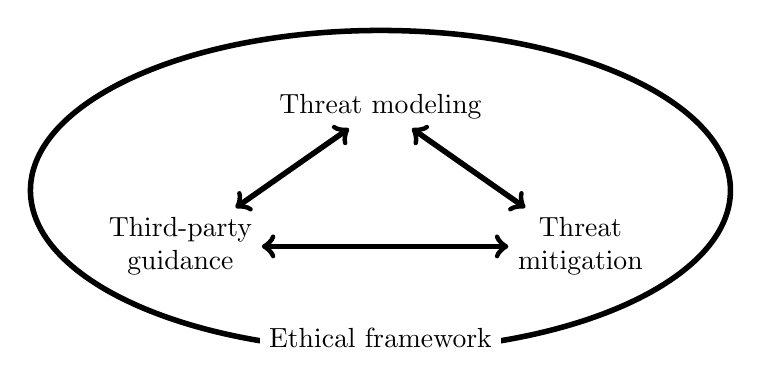
\begin{tikzpicture}[x = 1in, y = .7in]
\node (threatModeling) at (0,1) {Threat modeling};
\node[align=center] (threatMitigation) at (1,0) {Threat\\mitigation};
\node[align=center] (third) at (-1,0) {Third-party\\guidance};
% Triangle edges
\draw[<->,line width = 2pt] (threatModeling) -- (threatMitigation);
\draw[<->,line width = 2pt] (third) -- (threatMitigation);
\draw[<->,line width = 2pt] (third) -- (threatModeling);
\draw[line width = 2pt] (0,.4) ellipse (1.75in and .8in);
\node[fill=white] at (0, -.65) {Ethical framework};
\end{tikzpicture}
\end{center}
\end{frame}

\begin{frame}{Decision time}
\begin{enumerate} \pause
\item Already have IRB approval. \pause
\item Stepped back. Are we comfortable proceeding? \pause
\item Central organizers proposed proceeding \pause
\item Board of Advisers agreed \pause
\item Pilot test in a machine learning class (early spring 2017) \pause
\item Full-scale launch (mid-spring 2017) \pause
\item Continuous consideration overseen by Board of Advisers
\end{enumerate}
\end{frame}

\begin{frame}
\begin{figure}
\centering
\includegraphics[width=.8\textwidth]{figures/tensionFig}
\end{figure}
\end{frame}

\begin{frame}{Privacy, ethics, and data access: Generalizable principles}
\begin{center}
\Large \bblue{Key elements} of our process may help promote the \bgreen{ethical use of other data sources} by future researchers.
\end{center}
\begin{center}
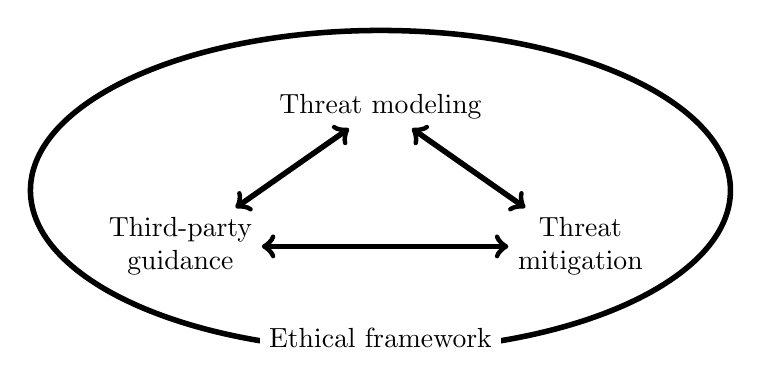
\begin{tikzpicture}[x = 1in, y = .7in]
\node (threatModeling) at (0,1) {Threat modeling};
\node[align=center] (threatMitigation) at (1,0) {Threat\\mitigation};
\node[align=center] (third) at (-1,0) {Third-party\\guidance};
% Triangle edges
\draw[<->,line width = 2pt] (threatModeling) -- (threatMitigation);
\draw[<->,line width = 2pt] (third) -- (threatMitigation);
\draw[<->,line width = 2pt] (third) -- (threatModeling);
\draw[line width = 2pt] (0,.4) ellipse (1.75in and .8in);
\node[fill=white] at (0, -.65) {Ethical framework};
\end{tikzpicture}
\end{center}
\end{frame}

\end{document}




%% DETAILED SLIDES ON MITIGATIONS ARE BELOW
\begin{frame}{Careful language}

What would happen if hundreds of social scientists and data scientists \only<1-1>{worked together}\only<2->{\blue{worked together}} on a \only<1-2>{scientific challenge}\only<3->{\blue{scientific challenge}} to \only<1-3>{improve the lives of disadvantaged children}\only<4->{\blue{improve the lives of disadvantaged children}} in the United States? \vskip .5cm
\onslide<5->{

\begin{center}[Statement about consent and IRB oversight]\end{center}

We have also taken \only<5-5>{further steps}\only<6->{\green{further steps}} to protect the participants in the Fragile Families and Child Wellbeing Study. \only<5-6>{If you would like to know more, please send us an email.}\only<7->{\green{If you would like to know more, please send us an email.}}}
\end{frame}

\begin{frame}
\centering
\huge \bblue{Generalizable principles}\vskip .5cm
\begin{itemize}
\item Do not overstate claims to have protected privacy. \vskip .3cm
\item Invite adversaries to become collaborators.
\end{itemize}
\end{frame}

\mitigations

\begin{frame}
\resizebox{1.1\textwidth}{!}{
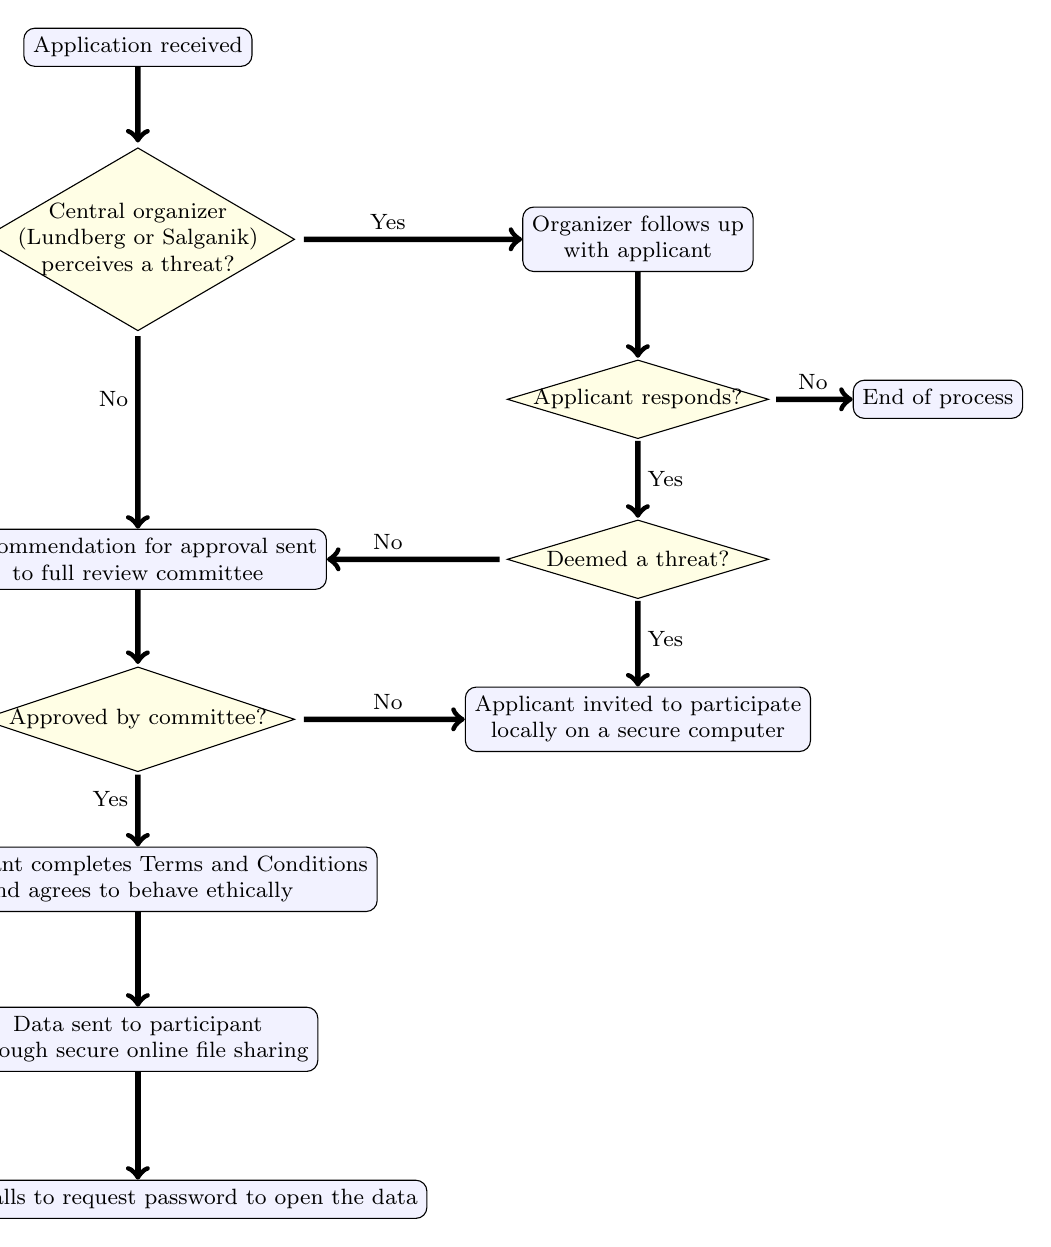
\begin{tikzpicture}[x = 2.5in, y = .8in,every node/.style={font=\footnotesize},trim left=-1.4cm]
\node[align=center,draw,rounded corners,fill=blue,fill opacity=.05,text opacity = 1] (apply) at (0,.2) {Application received};
\node[align=center,rectangle,draw,yscale=7,xscale = 12,rotate=45,fill=yellow,fill opacity=.1,text opacity = 1] (review1) at (0,-1) {};
\node[align=center] at (0,-1) {Central organizer\\(Lundberg or Salganik)\\perceives a threat?};
\node[align=center,anchor=south] at (.5,-1) {Yes};
\node[align=center,anchor = east] at (0,-2) {No};
\node[align=center,draw,rounded corners,fill=blue,fill opacity=.05,text opacity = 1] (flags) at (1,-1) {Organizer follows up\\with applicant};
\node[align=center,rectangle,draw,yscale=3,xscale = 10,rotate=45,fill=yellow,fill opacity=.1,text opacity = 1] (response) at (1,-2) {};
\node[align=center] at (1,-2) {Applicant responds?};
\node[anchor = west] at (1,-2.5) {Yes};
\node[anchor = south] at (1.35,-2) {No};
\node[align=center,draw,rounded corners,fill=blue,fill opacity=.05,text opacity = 1] (noResponse) at (1.6,-2) {End of process};
\node[align=center,rectangle,draw,yscale=3,xscale = 10,rotate=45,fill=yellow,fill opacity=.1,text opacity = 1] (realThreat) at (1,-3) {};
\node[align=center] at (1,-3) {Deemed a threat?};
\node[align=center,anchor=south] at (.5,-3) {No};
\node[align=center,anchor=west] at (1,-3.5) {Yes};
\node[align=center,draw,rounded corners,fill=blue,fill opacity=.05,text opacity = 1] (local) at (1,-4) {Applicant invited to participate\\locally on a secure computer};
\node[align=center,draw,rounded corners,fill=blue,fill opacity=.05,text opacity = 1] (recommendation) at (0,-3) {Recommendation for approval sent\\to full review committee};
\node[align=center,rectangle,draw,yscale=4,xscale = 12,rotate=45,fill=yellow,fill opacity=.1,text opacity = 1] (approved) at (0,-4) {};
\node[align=center] at (0,-4) {Approved by committee?};
\node[align=center,anchor = east] at (0,-4.5) {Yes};
\node[align=center,anchor = south] at (0.5,-4) {No};
\node[align=center,draw,rounded corners,fill=blue,fill opacity=.05,text opacity = 1] (terms) at (0,-5) {Participant completes Terms and Conditions\\and agrees to behave ethically};
\node[align=center,draw,rounded corners,fill=blue,fill opacity=.05,text opacity = 1] (data) at (0,-6) {Data sent to participant\\through secure online file sharing};
\node[align=center,draw,rounded corners,fill=blue,fill opacity=.05,text opacity = 1] (call) at (0,-7) {Participant calls to request password to open the data};
\draw[->, line width=2pt] (apply) -- (review1);
\draw[->, line width=2pt] (review1) -- (flags);
\draw[->, line width=2pt] (flags) -- (response);
\draw[->, line width=2pt] (response) -- (noResponse);
\draw[->, line width=2pt] (response) -- (realThreat);
\draw[->, line width=2pt] (realThreat) -- (local);
\draw[->, line width=2pt] (realThreat) -- (recommendation);
\draw[->, line width=2pt] (review1) -- (recommendation);
\draw[->, line width=2pt] (recommendation) -- (approved);
\draw[->, line width=2pt] (approved) -- (terms);
\draw[->, line width=2pt] (approved) -- (local);
\draw[->, line width=2pt] (terms) -- (data);
\draw[->, line width=2pt] (data) -- (call);
\end{tikzpicture}
}
\end{frame}

\begin{frame}
\centering
\resizebox{!}{.8\textheight}{
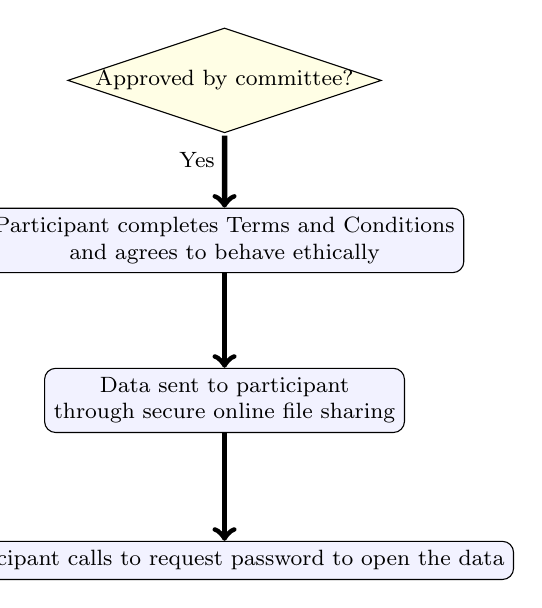
\begin{tikzpicture}[x = 2.5in, y = .8in,every node/.style={font=\footnotesize},trim left=-2.5cm]
\node[align=center,rectangle,draw,yscale=4,xscale = 12,rotate=45,fill=yellow,fill opacity=.1,text opacity = 1] (approved) at (0,-4) {};
\node[align=center] at (0,-4) {Approved by committee?};
\node[align=center,anchor = east] at (0,-4.5) {Yes};
\node[align=center,draw,rounded corners,fill=blue,fill opacity=.05,text opacity = 1] (terms) at (0,-5) {Participant completes Terms and Conditions\\and agrees to behave ethically};
\node[align=center,draw,rounded corners,fill=blue,fill opacity=.05,text opacity = 1] (data) at (0,-6) {Data sent to participant\\through secure online file sharing};
\node[align=center,draw,rounded corners,fill=blue,fill opacity=.05,text opacity = 1] (call) at (0,-7) {Participant calls to request password to open the data};
\draw[->, line width=2pt] (approved) -- (terms);
\draw[->, line width=2pt] (terms) -- (data);
\draw[->, line width=2pt] (data) -- (call);
\end{tikzpicture}
}
\end{frame}

\begin{frame}
\centering
\huge \bblue{Generalizable principle}\vskip .2cm Share data only with those likely to contribute.
\end{frame}

\mitigations

\begin{frame}{Ethical appeal}
The Fragile Families and Child Wellbeing Study \only<1-1>{is a dataset of real people who have selflessly opened up their lives to us}\only<2->{\blue{is a dataset of real people who have selflessly opened up their lives to us}} for the last 15 years so that their experiences can contribute to scientific research. By participating in the Fragile Families Challenge, you become a collaborator in this project. It is of the utmost importance that you \only<1-2>{respect the families}\only<3->{\blue{respect the families}} in the data by using what they have told us responsibly.
\end{frame}

\begin{frame}
\centering
\huge \bblue{Generalizable principle}\vskip .2cm Embed data sharing within norms of appropriate behavior.
\end{frame}

\mitigations

\begin{frame}
\resizebox{!}{.8\textheight}{
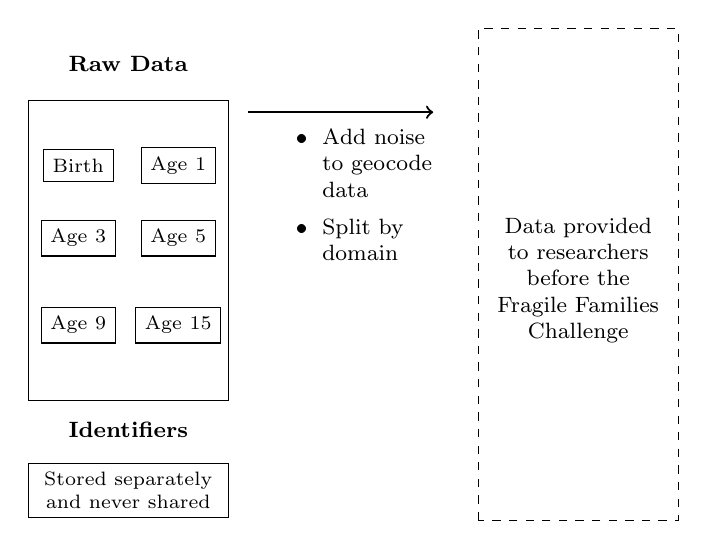
\begin{tikzpicture}[x = .5in, y = .6in, style={font=\footnotesize}]
% Raw data
\draw (-13, 0) rectangle (-11,2.5);
\node[align=center] at (-12, 2.8) {\textbf{Raw Data}};
\node[draw=black] at (-12.5, 1.955) {\scriptsize Birth};
\node[draw=black] at (-11.5, 1.955) {\scriptsize Age 1};
\node[draw=black] at (-12.5, 1.35) {\scriptsize Age 3};
\node[draw=black] at (-11.5, 1.35) {\scriptsize Age 5};
\node[draw=black] at (-12.5, 0.625) {\scriptsize Age 9};
\node[draw=black] at (-11.5, 0.625) {\scriptsize Age 15};
% Identifiers
\node[align=center] at (-12, -.25) {\textbf{Identifiers}};
\node[draw, align=center, font = \scriptsize, minimum width = 1in] at (-12, -.75) {Stored separately\\and never shared};
% Raw -> restricted arrow
\draw[thick, ->] (-10.8,2.4) -- (-8.95,2.4);
\node[text width = 1in,anchor = north] at (-9.75,2.5) {\begin{itemize}
\item Add noise to geocode data
\item Split by domain
\end{itemize}};
% Existing data rectangle
\draw[dashed] (-8.5, -1) rectangle (-6.5, 3.1);
\node[align=center] at (-7.5, 1) {Data provided\\to researchers\\before the\\Fragile Families\\Challenge};
\end{tikzpicture}
}
\end{frame}

\begin{frame}
\resizebox{!}{.8\textheight}{
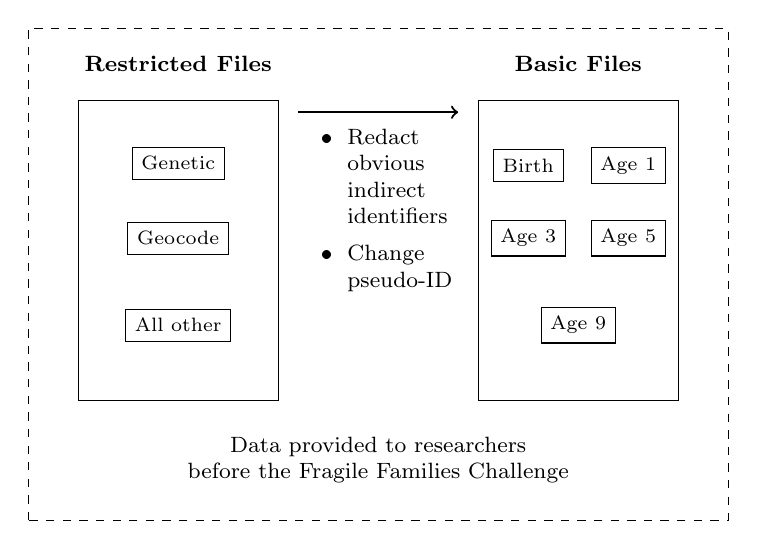
\begin{tikzpicture}[x = .5in, y = .6in, style={font=\footnotesize}]
% Existing data rectangle
\draw[dashed] (-8.5, -1) rectangle (-1.5, 3.1);
\node[align=center] at (-5, -.5) {Data provided to researchers\\before the Fragile Families Challenge};
% Restricted data
\draw (-8, 0) rectangle (-6,2.5);
\node[draw=black] at (-7, 1.975) {\scriptsize Genetic};
\node[draw=black] at (-7, 1.35) {\scriptsize Geocode};
\node[draw=black] at (-7, .625) {\scriptsize All other};
\node[align=center] at (-7, 2.8) {\textbf{Restricted Files}};
% Restricted -> public arrow
\draw[thick, ->] (-5.8,2.4) -- (-4.2,2.4);
\node[text width = .9in,anchor = north] at (-5.1,2.5) {\begin{itemize}
\item Redact obvious indirect identifiers
\item Change pseudo-ID
\end{itemize}};
% Public data
\node[align=center] at (-3, 2.8) {\textbf{Basic Files}};
\draw (-4, 0) rectangle (-2, 2.5);
\node[draw=black] at (-3.5, 1.955) {\scriptsize Birth};
\node[draw=black] at (-2.5, 1.955) {\scriptsize Age 1};
\node[draw=black] at (-3.5, 1.35) {\scriptsize Age 3};
\node[draw=black] at (-2.5, 1.35) {\scriptsize Age 5};
\node[draw=black] at (-3, 0.625) {\scriptsize Age 9};
\end{tikzpicture}
}
\end{frame}

\begin{frame}
\resizebox{!}{.8\textheight}{
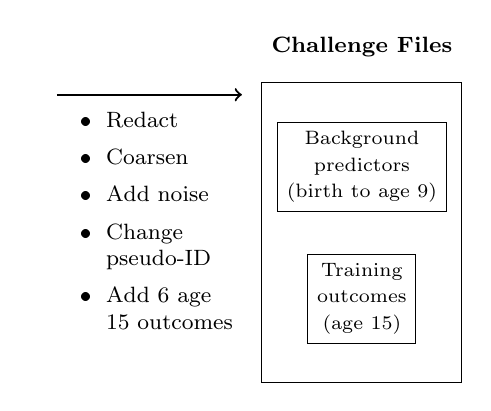
\begin{tikzpicture}[x = .5in, y = .6in, style={font=\footnotesize}]
% Public -> challenge arrow
\draw[thick, ->] (-1.05,2.4) -- (.8,2.4);
\node[text width = 1in,anchor = north] at (-.25,2.5) {\begin{itemize}
\item Redact
\item Coarsen 
\item Add noise
\item Change pseudo-ID
\item Add 6 age 15 outcomes
\end{itemize}};
% Challenge data
\node[align=center] at (2, 2.8) {\textbf{Challenge Files}};
\draw (1, 0) rectangle (3, 2.5);
\node[draw=black,align=center] at (2, 1.8) {\scriptsize Background\\\scriptsize predictors\\ \scriptsize(birth to age 9)};
\node[draw=black,align=center] at (2, 0.7) {\scriptsize Training\\\scriptsize outcomes\\\scriptsize(age 15)};
\end{tikzpicture}
}
\end{frame}

\begin{frame}
\centering
\huge \bblue{Generalizable principle}\vskip .2cm Only share the data needed for the research project.
\end{frame}

\mitigations
